\newpage
\section{Aufgabe 1}
\subsection{Aufgabenstellung}
Installieren Sie auf einer der beiden virtuellen Maschinen, die Sie fur Praktikum Nr. 1 eingerichtet haben, einen Webserver und eine Datenbank Ihrer Wahl (z.B. Apache, MySQL o.a.). Protokollieren Sie Ihr Vorgehen mithilfe der Vorlage.
\begin{enumerate}[label=(\alph*)]
	\item Welche Ports verwenden die Programme zur Kommunikation? Wie ändert man die Standardeinstellungen?Ist dazu ein Neustart des Systems nötig?
	\item Richten Sie eine restriktive Firewall ein (prohibitive Sicherheitspolitik). Es soll sichergestellt werden, dass ausschließlich der Port des Webservers von außen zugänglich ist. Die Firewall soll automatisch beim Start des Systems geladen werden. Nutzen Sie fur die Lösung der Aufgabe ausschließlich die Kommandozeile und das Kommando iptables.
	\item Nun soll wireshark verwendet werden. Pingen sie einen Rechner an und beobachten Sie den Netzwerkverkehr. Was geschieht, wenn Sie folgende Filterregel eingeben: iptables -A INPUT -p icmp -j DROP Wiederholen Sie den Vorgang mit der Policy REJECT. Was fällt auf? Wo sind die Unterschiede von DROP und REJECT, welche Vor- und Nachteile bieten sie jeweils? Löschen Sie nun wieder alle Regeln in iptables, setzen Sie die Policy zuruck ACCEPT auf und beenden Sie wireshark.
	\item Nun öffnen Sie mit netcat auf dem Rechner A (eine Ihrer VMs) ein oder zwei Ports zwischen 0 und 100. Nutzen Sie dafur den Befehl: nc -l [Portnummer] nmap ist ein Portscanner, mit dem man u.a. die eigene Firewall auf Sicherheitslücken testen kann. Mit nmap Zieladresse -p [Anfangsport]-[Endport] kann nach offenen Ports in einem bestimmten Portbereich gescannt werden. Fuhren Sie nun einen Portscan auf VM A von VM B aus. Welches Ergebnis sehen Sie?
	\item Definieren Sie nun Regeln mit iptables, die einen solchen Scan blocken. Dazu bietet es sich an, alle Pakete zu verwerfen, die ungewöhnlich schnell Verbindungsanfragen senden. Sehen Sie sich die folgende Regel an und versuchen Sie zu verstehen, welchen Sinn die einzelnen Befehle erfullen. Sie werden sie im Verlauf dieser Übung noch benötigen. Tipps: (www.snowman.net/projects/ipt recent). iptables -A INPUT -p tcp -i eth1 -m state --state NEW -m recent --set Wenden Sie diese Regel an. Die zweite Regel soll nun bei genau solchen Paketen in der gleichen Liste nachsehen, ob die Adresse eines Paketes bereits eingetragen ist. Trifft dies zu, soll die letzte Zeitmarke upgedatet werden. Wenn nun ein und dieselbe Adresse versucht 20 oder mehr Verbindungsanfragen innerhalb von 10 Sekunden zu senden, sollen all diese Pakete verworfen werden. Wie sieht die entsprechende Regel aus? Testen Sie die Funktionalit¨at der Regeln mit nmap.
	\item Nun sollen die Portscans mithilfe der LOG-Funktion protokolliert werden. Dazu kann zuerst eine neue Kette fur Portscans mit Namen PORTSCAN o. ä. erstellt werden. Als zweites muss eine Regel definiert werden, die alle Pakete in dieser Kette protokolliert. Als LogPrefix soll "PORTSCAN erkannt --" verwendet werden. iptables loggt i.d.R. in der Datei /var/log/syslog. Kontrollieren Sie, ob Ihre Ausgabe in der Logdatei erscheint.
	\item Hping3 ist ein Tool, um die eigene Firewall zu testen. Es kann benutzerdefinierte TCPPakete generieren und das auch mit langsamerer Geschwindigkeit als nmap. Schicken Sie einer VM mehrere TCP-Pakete mit gesetzter SYN-Flag beginnend bei Port 0. Welchen Befehl verwenden Sie und woran erkennt man, welche Ports offen sind?
\end{enumerate}

\subsection{Vorbereitung}
Installation von Apache und MySql auf einer der beiden VMs. Einlesen in die Doku von iptables.

\subsection{Durchführung}

\subsubsection{a)}
MySQL nutzt standardmäßig den \textbf{Port 3306}. Um bei MySQL den Port zu ändern muss man den Eintrag \textbf{port = 3360} in die /etc/mysql/mysql.conf.d/mysqld.cnf schreiben. Es reicht aus nach einer Änderung der Service neu zu starten. Apache lauscht an auf den \textbf{Ports 80} und \textbf{443}. Um dies zu ändern muss man, in der ports.conf, mit \textbf{Listen 200} angeben auf welchen Ports gelauscht werden soll.Mit \textbf{service apache2 reload} kann die Konfigurationsdatei neu geladen werden ohne den Service oder das System neu zu starten.

\subsubsection{b)}
Als erstes müssen wir alle bisherigen Einträge löschen
\begin{lstlisting}
sudo iptables -F
\end{lstlisting}
Nun sperren wir alle ein kommenden Verbindungen
\begin{lstlisting}
sudo iptables  -P INPUT DROP
sudo iptables  -P FORWARD DROP
\end{lstlisting}
Nun erlauben wir alle ausgehende Verbindungen 
\begin{lstlisting}
sudo iptables  -P OUTPUT ACCEPT 
\end{lstlisting}
Nun erlauben wir alle ein kommenden Verbindungen auf den \textbf{Port 80}
\begin{lstlisting}
sudo iptables -A INPUT -p tcp --dport 80 -j ACCEPT
\end{lstlisting}
Nun erlauben wir noch alle lokalen ein kommenden Verbindungen
\begin{lstlisting}
sudo iptables -A INPUT -j ACCEPT -s 127.0.0.1 
\end{lstlisting}
Nun müssen wir noch dafür sorgen das diese Regeln auch noch nach einem Neustart noch vorhanden sind
\begin{lstlisting}
sudo sh -c "iptables-save > /etc/firewall.conf"
\end{lstlisting}
\begin{lstlisting}
nano /etc/network/if-up.d/iptables
\end{lstlisting}
In diese Datei schreiben wir folgendes 
\begin{lstlisting}
iptables-restore < /etc/firewall.conf
\end{lstlisting}
Nun geben wir noch Ausführrechte für dieses Shell-Skript
\begin{lstlisting}
sudo chmod +x /etc/network/if-up.d/iptables
\end{lstlisting}

\subsubsection{c)}
Den ersten Ping führen mit \textbf{ping -c 1 <IP-Adresse>} aus. Dieser wird auch ohne Probleme ausgeführt.
\begin{lstlisting}
iptables -A INPUT -p icmp -j DROP
\end{lstlisting}
Nun funktioniert der Ping nicht mehr und wir haben Paketverlust.
Bei \textbf{REJECT} wird die Antwort ebenfalls nicht weitergeleitet aber zusätzlich
wird ein ICMP-Fehler Paket mit dem Code Port \textbf{unreachable} gesendet.\\\\
\textbf{DROP} bringt den Vorteil es schützt vor einen DoS-Angriff, weil er Verhält sich als würde es den Server nicht geben. \textbf{REJECT} gibt eine Rückmeldung und lässt den Client darauf reagieren und hilft beim debuggen.

\subsubsection{d)}
Als erstes öffnen unsere Ports mit \textbf{sudo nc -l <Port>}.
Wir öffnen die Ports 22 und 88. 
\begin{lstlisting}
sudo nc -l 22
sudo nc -l 88 
\end{lstlisting}
Nun installieren wir \textbf{nmap}
\begin{lstlisting}
sudo apt-get install nmap 
\end{lstlisting}
Nun horchen wir an allen Ports einer IP, von Rechner A(10.0.2.15).
\begin{lstlisting}
nmap 10.0.2.15 -p 0-100
\end{lstlisting}
\begin{figure}[H]
	\centering
	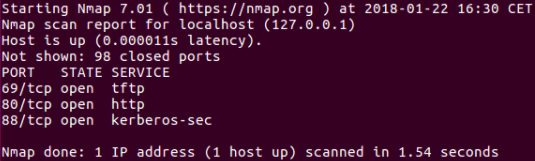
\includegraphics[width=0.8 \linewidth]{images/f01}
	\caption{nmap} \label{ordner}
\end{figure} 

\subsubsection{e)}
Die Regel:
\begin{lstlisting}
sudo iptables -A INPUT -p tcp -i enp0s8 -m state --state NEW -m recent --set
\end{lstlisting}
\begin{table}[h!]
  \begin{center}
  \caption{Erklärung der Parameter}
    \label{tab:table1}
    \begin{tabular}{l|r} 
      \textbf{Parameter} & \textbf{Bezeichnung}\\
      \hline
      -A INPUT & nur eingehende Pakete\\
      -p tcp & nur TCP-Pakete\\
      -i enp0s8 & nur an dieses Netzwerkinterface\\
      -m recent --set & Speichert den Absender wenn alles Bedingungen stimmen\\
    \end{tabular}
  \end{center}
\end{table}
	
Um diese Aufgabe lösen zu können benötigen wir das folgende Kommando
\begin{lstlisting}
iptables -A INPUT -m state --state NEW -m recent --update --seconds 10 --hitcount 20 -j DROP
\end{lstlisting}

\subsubsection{f)}
Als erstes müssen wir den Filter von Rechner A anpassen und eine neue Kette erstellen. 
\begin{lstlisting}
sudo iptables -N PORTSCAN
\end{lstlisting}
Jetzt definiere eine neue Regel zum protokollieren.
\begin{lstlisting}
sudo iptables -A PORTSCAN -m recent --name portscan --set -j LOG --log-prefix 'PORTSCAN erkannt --' --log-level debug
sudo iptables -A PORTSCAN -j DROP
\end{lstlisting}
Jetzt müssen wir nochmal dafür sorgen, dass bei zu vielen Anfragen an die oben erstellte Kette weitergeleitet werden. Die letzte Regel verwirft dann alle Pakete von deren Absender die in der portscan-Liste stehen.
\begin{lstlisting}
sudo iptables -A INPUT -p tcp -i enp0s8 -m state --state NEW -m recent --set
sudo iptables -A INPUT -p tcp -i enp0s8 -m state --state NEW -m recent --update --seconds 10 --hitcount 20 -j PORTSCAN
sudo iptables -A INPUT -m recent --name portscan --rcheck -j DROP
\end{lstlisting}

\subsubsection{g)}
Wir scannen als erstes die Ports:
\begin{lstlisting}
hping3 -V -S 192.168.56.102 -p -scan 0-100 -i u550000
\end{lstlisting}
Die eingestellte Wartezeit zwischen den Paketen (0.55 Sekunden) sorgt dafür, dass der Scan von den in der vorherigen erstellten Regeln nicht wirken.

\subsection{Fazit}
Diese Aufgabe hatte keine Probleme.
